\documentclass[12pt,letterpaper]{lsuetd}
\usepackage{setspace,graphics,dsfont,verbatim,paralist,indentfirst,amsmath}
\usepackage{tabularx}
\usepackage{empheq}
\usepackage{color}
\usepackage[table]{xcolor}
\usepackage{colortbl}
\usepackage{rotating}
\usepackage{fancyref}
\setlength{\topmargin}{-0.5in}
\setlength{\textheight}{9.0in}
\addtolength{\evensidemargin}{-0.50in}
\addtolength{\oddsidemargin}{-0.50in}
\addtolength{\textwidth}{1.00in}
\setlength{\parindent}{1.75em}
\setlength{\parskip}{0ex}
\setcounter{tocdepth}{2}

\definecolor{Gray}{gray}{.9}
\newcommand\y{\cellcolor{gray!10}}


\usepackage{titlesec}

\usepackage{etoolbox}
\makeatletter
\patchcmd{\ttlh@hang}{\parindent\z@}{\parindent\z@\leavevmode}{}{}
\patchcmd{\ttlh@hang}{\noindent}{}{}{}
\makeatother

\titlespacing*{\section}
{0pt}{36pt}{24pt}
\titlespacing*{\subsection}
{0pt}{24pt}{18pt}
\titlespacing*{\subsubsection}
{0pt}{18pt}{12pt}

%\titleformat*{\subsubsection}{\large\bfseries\thesection.\thesubsection}
\titleformat*{\subsubsection}{\large\bfseries}

\makeatletter

\begin{document}
\renewcommand\@pnumwidth{1.55em}
\renewcommand\@tocrmarg{9.55em}
\renewcommand*\l@chapter{\@dottedtocline{0}{1.5em}{2.3em}}
\renewcommand*\l@figure{\@dottedtocline{1}{0em}{3.1em}}
\let\l@table\l@figure

\pagenumbering{roman}
\thispagestyle{empty}
\begin{center}
%The title page is first created.
A GRAPH-BASED TAXONOMIC INTELLIGENT TUTORING SYSTEM UTILIZING 
BLOOM'S TAXONOMY AND ITEM-RESPONSE THEORETIC ASSESSMENT

\vfill
\doublespacing
A Thesis/Dissertation \\
\singlespacing
Submitted to the Graduate Faculty of the \\
Louisiana State University and \\
Agricultural and Mechanical College \\
in partial fulfillment of the \\
requirements for the degree of \\
Ph.D. \\
\doublespacing
in \\
                                       
Computer Science \\
\singlespacing
\vfill

by \\
Dennis Castleberry \\
B.S., LSU, 2009 \\
May 2017
\end{center}
\pagebreak
%The Copyright Page and Dedication sections can be added here, if desired.

%\chapter*{Copyright Page}
%\doublespacing
%\vspace{0.55ex}
%Insert the appropriate text for the copyright page here.
%\addcontentsline{toc}{chapter}{\hspace{-1.5em} {COPYRIGHT PAGE} \vspace{12pt}}
%\pagebreak

%\chapter*{Dedication}
%\doublespacing
%\vspace{0.55ex}
%Insert the appropriate text for the dedication or epigraph page here.  This part of the ETD must not exceed one page.
%\addcontentsline{toc}{chapter}{\hspace{-1.5em} {DEDICATION} \vspace{12pt}}
%\pagebreak

\chapter*{Acknowledgments}
\doublespacing
\vspace{0.55ex}

I would like to thank my research group, my committee, and the Department of
Computer Science for supporting my teaching and research efforts throughout
my career.

%The code below adds the Acknowledgments section to the Table of Contents.
\addcontentsline{toc}{chapter}{\hspace{-1.5em} {ACKNOWLEDGMENTS} \vspace{12pt}}
\pagebreak
%The Preface section can now be added, if desired.

%\chapter*{Preface}
%\doublespacing
%\vspace{0.55ex}
%Insert the appropriate text for the preface here.
%\addcontentsline{toc}{chapter}{\hspace{-1.5em} {PREFACE} \vspace{12pt}}
%\pagebreak

\singlespacing
\tableofcontents
\pagebreak

%The code below generates the List of Tables and adds it to the Table of Contents.
\renewcommand\@pnumwidth{1.55em}
\renewcommand\@tocrmarg{8.55em}
\addcontentsline{toc}{chapter}{\hspace{-1.5em} LIST OF TABLES \vspace{12pt}}
\listoftables
\pagebreak
%The code below generates the List of Figures and adds it to the Table of Contents.
\addcontentsline{toc}{chapter}{\hspace{-1.5em} LIST OF FIGURES \vspace{12pt}}
\listoffigures
\pagebreak
%The List of Nomenclature may be included here, if desired.

%\chapter*{List of Nomenclature}
%\doublespacing
%\vspace{0.55ex}
%Provide the definitions of the symbols used in your thesis or dissertation here.
%\addcontentsline{toc}{chapter}{\hspace{-1.5em} LIST OF NOMENCLATURE \vspace{12pt}}
%\pagebreak

%The code below adds the Abstract and places it within the Table of Contents.
\renewenvironment{abstract}{{\hspace{-2.2em} \huge \textbf{\abstractname}} \par}{\pagebreak}
\addcontentsline{toc}{chapter}{\hspace{-1.5em} ABSTRACT}
\begin{abstract}
\vspace{0.55ex}
\doublespacing
Insert the text of your abstract here.  Make sure there is one blank line between the end of the Abstract text and the ``end'' command below to maintain double--spaced lines.

\end{abstract}

\pagenumbering{arabic}
\addtocontents{toc}{\vspace{12pt} \hspace{-1.8em} CHAPTER \vspace{-1em}}
\singlespacing
\setlength{\textfloatsep}{12pt plus 2pt minus 2pt}
\setlength{\intextsep}{6pt plus 2pt minus 2pt}
\chapter{Background Information}
\doublespacing

\section{Bloom's Taxonomy}

\subsection{The Interpretation in Computer Science}
\subsection{Assumptions of this Work}

\section{Item Response Theory}

\subsection{Evaluation of Trait Ability}

\section{Factor Analysis}

\subsection{Confirmatory vs. Exploratory}
\subsection{Principal Axis Factoring}

\section{Previous Research}


\pagebreak
\singlespacing
\chapter{Items and Sets}
\doublespacing
\section{Representing Items}


The database contains items of the following nature:

\begin{itemize}

  \item \emph{Content}.  These include facts (which may be arranged into
  paragraphs, subsections, and sections), definitions, diagrams, and source
  codes.

  \item \emph{Assessment}.  These include questions, which may be true/false,
  multiple-choice, code writing, code simulation, short answer, and
  freewriting; also Likert scale items.

\end{itemize}

\subsection{Taxonomic Information}

Any output from this database to the student which is intended to solicit input
from the student has the following ordinal dimensions:

\begin{itemize}

  \item \emph{Difficulty}. Following the +/- grading system, difficulties range
  from -7 (very easy) to +7 (very hard), with 0 being medium. The difficulty
  indicates the probability that any given student in the class will answer the
  item correctly.

  \item \emph{Bloom level}.  The Bloom levels of cognitive functioning are
  Knowledge, Comprehension, Application, Analysis, Evaluation, and Synthesis.

  \item \emph{Concept}.  Concepts are covered in an elementary C++
  programming course, and include: Variables, Expressions, Control Structures,
  etc.

\end{itemize}

Any output to the student also has the following categorial dimensions:

\begin{itemize}

  \item \emph{Context}.  A problem may have a domain-specific context, e.g. it
  may be a problem relevant to biology, chemistry, physics, mathematics, etc.

  \item \emph{Type}.  The problem may be true/false, multiple-choice, code
  writing, code simulation, short answer, or freewriting.

\end{itemize}

Each output may also have a dependency list, that is a list of IDs of, or a
rule describing, other output entries which the student should be exposed to
prior to that output.  It is important to note that the dimensions of the data
are not limited to the above; an exploratory factor analysis has the potential
to extend the dimensionality of the data semi-automatically.  For the moment,
Bloom level, subject domain, concept, and difficulty are dimensions of a test
question.  Exploratory factor analysis gives loadings of some $n$ number of
factors which are hypothesized to account for the variance in the data.  Thus
it could potentially find a factor other than one listed which accounts for a
significant amount of variance. In that case, the instructor could interpret
the loading matrix and label the levels of the factor accordingly.

\subsubsection{Examples of Content Items}

What follows is example output which does not aim to solicit input, but rather
inform the user (content).  Below is a definition of a compiler output.

\begin{quote}
[Definition 1]: compiler: a program which generates an executable from a source
code
\end{quote}

Likewise, below is a fact which has as one of its dependencies the definition
of a compiler, given above.

\begin{quote}
[Fact 1]: A compiler is itself a program.
\end{quote}

In a content schedule, Fact 1 has Definition 1 as a dependency. Therefore in
any schedule including Fact 1, Definition 1 will be included unless an
assessment response set shows that Definition 1 is known.

\subsubsection{Measuring Trait Ability}

To form a statistical basis for content scheduling, the measure of trait
ability should be done per-concept and Bloom level.  For each $i^{th}$
question, the trait ability estimation should take into account:

\begin{itemize}

  \item the probability of guessing the question correctly, $\gamma_i$,

  \item the item discrimination $\alpha_i$, or to what extent the question
        distinguishes good from poor trait ability for the concept,

  \item the difficulty $\beta_i$, including the question difficulty \emph{as
        such}

  \item the propensity of trait level to change over time.

  \end{itemize}

Trait ability will be measured using (a possibly modified form of) IRT.  In
contrast to CTT---in which the meaning of a composite test score is interpreted
by comparing it to the mean of composite scores obtained from the same
sample--- IRT obtains meaning of test results by computing the likelihood that
the student could answer the questions in the way he or she did assuming a
trait ability.  In CTT, for a standardized test, one may calculate the z-score
for a composite test score as follows:

\[
  z = \frac{x - \mu}{\sigma}.
\]
%\todo{Is z-score a per trait thing? a per bloom level thing?}
%\response{The z-score is calculated from composite test scores. It tells how
%many standard deviations above or below the mean a composite score is.}

The $z$-score gives the number of standard deviations from the mean.  $-1 < z <
l$ average, $z > 1$ is above average, and $z < -1$ is below average.  One may
score the test accordingly.  Some instructors use a more intuitive approach,
graphing the distribution and clustering the data, to identify distinct
clusters of scores.  However, neither measure of trait ability accounts for the
considerations above (unless item discrimination was ensured by using a factor
analysis to design the test). 

In IRT, the trait ability is measured using a formula expressing the
probability that the student $s$ will answer the item $i$ correctly
\cite{embretson2000}: 

\[
 P(X_{is}=1 | \theta_s, \alpha_i, \beta_i, \gamma_i) = 
 \gamma_i + (1-\gamma_i) 
 \frac{    e^{\alpha_{i}(\theta_{s} - \beta_{i})}}
      {1 + e^{\alpha_{i}(\theta_{s} - \beta_{i})}}
\]

Suppose the student's response vector is $y_s$, where $y_{is}$ is the student's
response to the $i^{th}$ question.  $y_{is}$ is 0 if the answer is incorrect,
and 1 otherwise.  If the trait ability $\theta_s$ is not known, then it may be
estimated by searching the hypothesis space of $\theta_s$ for the probability
which maximizes $\prod^m P(y_{is})$, that is the product of probabilities that
$s$ answers each of the $m$ total questions for that question in the manner
he or she did.  That is, we seek the $\theta_s$ which maximizes the probility
of the student's response set:

\[
 \underset{\theta_s}{\textrm{argmax}}
 \prod^m
 \Bigg[
 \gamma_i + (1-\gamma_i) 
 \frac{    e^{\alpha_{i}(\theta_{s} - \beta_{i})}}
      {1 + e^{\alpha_{i}(\theta_{s} - \beta_{i})}}
 \Bigg].
\]

To find this trait ability, we may use a gradient descent method on the above
function of $\theta_s$ until convergence to a satisfactory precision required
to assign a letter grade (1e-1) \cite{embretson2000}. 

\subsection{Dependency Information}

\section{Representing Assessments}

\subsection{Graph Structure}

\pagebreak
\singlespacing
\chapter{Trait Ability}
\doublespacing
\section{Representing Ability}

To form a statistical basis for content scheduling, the measure of trait
ability should be done per-concept and Bloom level.  Therefore if there are $m$
concepts and $n$ levels, there are then $nm$ number of $\theta$ values.  This
shall be called $\Theta$, the trait ability matrix; and $\Theta_s$ will denote
the trait ability matrix of student $s$.  Let $j$ be the index of a Bloom level
and $k$ be the index of a concept, then:

\begin{equations}
\Theta_s =\left[
         \begin{array}{lllll}
              \theta_{s11} & \ldots       & \ldots       & \ldots & \theta_{sn1}  \\
              \vdots       & \ddots       &              &        &               \\
              \vdots       &              & \theta_{sjk} &        &               \\
              \vdots       &              &              & \ddots &               \\
              \theta_{s1m} &              &              &        & \theta_{snm}  \\
         \end{array}
       \right]
\end{equations}

While not strict, there is certainly an ordering about $\Theta$. Lower-level
concepts come before higher-level concepts, and lower Bloom levels come before
higher Bloom levels.  Conceivably a $\Theta$ may look like the following:

\begin{equations}
\Theta_1 =\left[
         \begin{array}{llllll}
             3 & 2.5 & 1   & \y0 & -1     & -2   \\
             2 & 1.5 & \y0 & -.5 & -1.5   & -2.5 \\
             1 &  .5 & \y0 & -1  & -2     & -3   \\
             1 & \y0 & -.5 & -1  & -2.5   & -3   \\
         \end{array}
       \right]
\end{equations}
\vspace{12pt}

Highlighted are areas where $\theta_{sjk} = 0$. These are the areas where the
student has roughly .5 probability of answering a question at difficulty
$\beta=0$ correctly.  Now the question arises: given a rich content item set
with questions in all (Bloom $\times$ concept $\times$ difficulty) categories,
which categories should be selected?  Many factors are taken into account.

\section{Proximal Zone of Development}

Clearly the higher $\theta_{sjk}$ values should be left alone, particularly
those nearing 3, since this demonstrates exceptional mastery of that (Bloom
$\times$ concept) category.  In particular, if $\theta_{sjk} = 3$, there is no
sense in asking at all since trait abilities are capped at 3.  In probabilistic
terms and relative to questions, asking questions for which the estimated
probably is overwhelmingly high, for example $p > .9$, serves no purpose, since
probability estimates of that degree require $\theta-\beta$ significantly
greater than 0.

% TODO: (SRB) What does the x in $\theta_{sjk} = x$ mean? Is it a question
% difficulty?  
If $\theta_{sjk} = x$, that is if the difficulty per student, Bloom level and
concept is some value $x$, then it would be ``unfair'' to ask questions in that
category which have $\beta > x$.  According to Equation~\ref{eq:irt}, if $\beta
> x$ and $\theta_{sjk} < x$, then $\theta{sjk}-\beta < 0$ and therefore
$p(\theta_{sjk}) < .5$, which means the student has less than .5 probability to
answer correctly.  Asking questions for which $p(\theta_{sjk}) < .5$ has
psychological ramifications, and potential problems for the updated MLE of
$\theta_{sjk}$.

It is true that correct answers of more challenging questions raise the ability
returned by a maximum likelihood estimate, however if the probability of
answering them is consistently less than chance and the student responds
accordingly, it is unlikely the estimate will return any $\theta_{sjk} > x$ for
those problems.  Also, given the information $\Theta_s$ about the student, if
it is known that the particular student will more than likely fail a particular
question, it would not make sense to ask it from a psychological standpoint,
provided that the intention of asking is to raise trait ability levels.  If the
student consistently experiences more failures than successes, the student is
more likely to be discouraged by the testing. 
%citation

There is another consideration: the concept tier and Bloom levels.  The course
is a progression of concepts across Bloom levels.  There is evidence to suggest
that students prefer problems with Bloom levels as high as they are able to
solve \cite{goel2004}; and ideally, the student should see steady progress in the
concepts of the course.  The set of questions asked at any given time in a course of study
typically range over a subset of concepts.  Testing for all concepts begins at
the Knowledge level; as new concepts are introduced over time, the tested Bloom
level for earlier-introduced concepts rises.  In a ``perfect'' situation, we
might observe a trait ability matrix as in Equation~\ref{eq:perfect}, which
shows a clear diagonal reflecting a progression in both concepts and Bloom
levels.  

\begin{equations}
\label{eq:perfect}
\Theta_2 =\left[
         \begin{array}{llllll}
             3   & 3   & 2   &  1 & \y0\\
             3   & 2   & 1   &\y0 & -1 \\
             2   & 1   & \y0 & -1 & -2 \\
             1   & \y0 & -1  & -2 & -3 \\
             \y0 & -1  & -2  & -3 & -3 \\
         \end{array}
       \right]
\end{equations}
\vspace{12pt}

With all this in mind, the most logical subset of (Bloom $\times$ concept)
categories to select questions from are those in the neighborhood of
$\theta_{sjk} = 0$.  One interpretation of this subset is that it is the
student's proximal zone of development.  In the psychology of learning, the
proximal zone of development is the area or areas in which a student can
perform a task with assistance, but could not perform the task without
assistance.  This is consistent with $p \approx .5$.
% citation

However, any question can potentially be asked for any (Bloom $\times$ concept)
category while still placing $p$ at or just slightly above .5 by manipulating
difficulty.  In fact, a matrix of difficulties for desired target questions
could be calculated from the ability matrix:

\begin{equations}
  B_s = \Theta_s - \delta
\end{equations}

where $\delta$ is a sufficiently low value, such as .5.  In the case of
student $s=1$, $B$ would then equal:

\begin{equations}
B_1 =\left[
         \begin{array}{llllll}
             2.5 & 2    & 1   & -.5  & -1.5   & -2.5 \\
             1.5 & 1.5  & -.5 & -1   & -2     & -3   \\
             .5  &  0   & -.5 & -1.5 & -2.5   & -3.5 \\
             .5  & -.5  & -1  & -1.5 & -3     & -3.5 \\
         \end{array}
       \right]
\end{equations}
\vspace{12pt}

% FIXME
% TODO: (SRB) I have trouble following the next paragraph
Then, it is possible to threshold the matrix so as to eliminate the [Bloom
$\times$ concept] categories after this stepladder, but include some lag up to
and not including those $\beta_{sjk}$ values for which the student has
$\theta_{sjk}$ indicating distinguished mastery:

\begin{equations}
B_1 =\left[
         \begin{array}{llllll}
                 & 2    & 1   & -.5  &        &      \\
             1.5 & 1.5  & -.5 &      &        &      \\
             .5  &  0   & -.5 &      &        &      \\
             .5  & -.5  &     &      &        &      \\
         \end{array}
       \right]
\end{equations}
\vspace{12pt}

From here, the density of questions asked may be in proportion to the distance
from -.5.  Eventually, either the student will reach $\theta_{sjk} = 3$ or else
the tutoring system will run out of questions for that (Bloom $\times$
concept), in which event the trait ability level will stay.

Sometimes the trait ability matrix may be jagged:

\begin{equations}
\Theta_1 =\left[
         \begin{array}{llllll}
             3 & 3   & 2   & \y0  & -1     & -2   \\
             3 & 2.5 & 1   & \y-.5  & -1.5   & -2.5 \\
             3 & 3   & 2.5 & \y-1 & -2     & -3   \\
             2 & 1.5 & \y-.5 & -1   & -2.5   & -3   \\
         \end{array}
       \right]
\end{equations}
\vspace{12pt}

in which event, the scheduler discussed in Sec~\ref{sec:scheduler} will attempt
to correct the trait ability matrix by asking questions in such a manner as to
have the proximal zone of development conform to a diagonal shape, which is
consistent with a smooth progression across Bloom levels and concepts.

It is possible, in fact, to have a three-dimensional structure as depicted in
Fig~\ref{fig:lattice}.  In the original conception of this work, the schedular
was intended to support not only progressions along the (concept $\times$
Bloom) categories, but also to identify subdomains of interest.
Introductory-level computer science invites many creative opportunities for
assigning interdisciplinary problems; for example coding problems related to
biology, chemistry, physics, mathematics, and even digital art.  It was assumed
that assigning problems catering to the students' interests would raise the
incentive to learn the concept.  

While the features of the scheduler were not extended to support the capability
to ``zero in'' on the student's domain-specific interests, the database problem
taxonomy supports tagging problems by subdomain.  The trait ability matrix may
be extruded to include this interest dimension.

\begin{figure}[p!]
 \label{fig:lattice}
 \includegraphics[width=\textwidth]{fig/lattice.eps} 
 \caption{The trait ability lattice, which accounts for domain-specific 
  interests}
\end{figure}

This structure, $\Theta$, therefore shows where to begin asking questions.  It
also helps to define the goal of the intelligent tutoring system: to increase
values in $\Theta$ successively along its diagonal, thereby engineering an
experience similar to course progression.
% FIXME

\section{Updating Ability}

The trait ability matrix must be refreshed (either after a student response,
for a more fine-grained scheduling, or after a total assessment for
coarse-grained scheduling).  Therefore the student responses must be
auto-graded, and an MLE for each element in $\Theta$ must be performed.

\subsection{Short Answer}

For short answer questions, $\gamma$ is set to 0, since it is assumed that
there are infinitely many possible responses to the short answer question,
unless otherwise indicated in the problem specification. 

Support for auto-grading short answer questions was easily obtained.  Short
answer questions can be graded using the Levenshtein distance, also known as
the edit distance.  Essentially, the Levenshtein distance gives the number of
edits (insertions, substitutions and deletions) required to arrive from the
student input to the solution.  If the Levenshtein distance is below a
threshold, the answer is marked correct; otherwise it is marked incorrect. 
% TODO: (SRB) my experience with Levenshtein distance is that it rarely
% performs as well as counting the number of letters in common.

% FIXME
% Jaro-Winkler distance
% Sorensen-Dice coefficient
% overlap coefficient

\subsection{Coding}

An independent component for auto-grading code does exist, but it has not been
integrated into the system.  The code auto-grader uses a humble approach; it
associates expressions from the Piraha language \cite{piraha} with point values:
% TODO: (SRB) A regex or a Piraha expression?
% FIXME: The original implementation does in fact use Piraha expressions.

 \begin{align*}
  \langle expr \rangle_1 & \rightarrow  x_1 \\
  \langle expr \rangle_2 & \rightarrow  x_2 \\
                         & \vdots       \\
  \langle expr \rangle_i & \rightarrow  x_i \\
                         & \vdots       \\
  \langle expr \rangle_n & \rightarrow  x_n 
 \end{align*}

where $\langle expr \rangle_i$ is some regular expression, and $x_i$ is the
point value assigned, which may be negative.  This is to dock for the
appearance of certain constructs.

The problem is scored based upon the expressions which were parsed, allowing
a minimum score no greater than zero:

\begin{equation}
  \max \Bigg\{ \displaystyle\sum_{i=1}^n x_i, 0 \Bigg\}
\end{equation}



\pagebreak
\singlespacing
\chapter{Item Dependencies}
\doublespacing
\section{Dependency Information}

No representation of trait ability mentioned so far specifically accounts for
dependency relationships between questions.  There are certainly dependency
relationships between whole (Bloom $\times$ concept) catogories.  For example,
one must be able to execute a for-loop (Comprehension of Loops) well before
gaining the ability to write one which satisfies an intended goal (Synthesis of
Loops). This is a course-grained dependency.

Other course-grained dependencies might be less obvious; questions in
categories for which concept is high-level and Bloom is low-level, depending on
questions in categories for which concept is lower-level and Bloom is
high-level.  For example, understanding a for-loop (Comprehension of Loops) is
predicated on being able to evaluate expressions (Application of Expressions).
In a trait ability matrix, these categories might even lie on a diagonal, which
would otherwise seem to suggest their independence.

Consider finer-grained dependency relationships among the following specific
questions regarding expressions:

\begin{verbatim}
 (a) What is (5 % 2)?
 (b) What is (5 / 2)?
 (c) What is (5 % (5 / 2))?
\end{verbatim}

The intuition captured by this example is that Part (c) could not be answered
correctly, at least not by any logical chain of reasoning, without possessing
the specific application ability that Part (a) and Part (b) test for.

It is probably true that Part (c) is more difficult than Part (a) or Part (b),
but this is not the reason for the dependency; rather it would appear the
dependency is the reason for the higher difficulty.  In terms of questions
which test application ability for expressions, all of the questions are in the
same neighborhood of difficulty; it is even possible albeit unlikely for the
$\beta$ values for all of these to be equal.  

However, if dependencies of the form $c \rightarrow a$ and $c \rightarrow b$
exist (that is, $c$ depends on $a$ and $b$), they may be indicated by a
high simple matching coefficient:

\begin{table}
 \caption{Notation for counts of joint observations}
 \vspace{12pt}
 \begin{tabularx}{\textwidth}{|X|X|X|X|}
 \hline
        & \y $y=0$         & \y $y=1$         & \y total     \\ \hline
  \y $x=0$ & $n_{00}$      & $n_{01}$      & $n_{0 \bullet }$  \\ \hline
  \y $x=1$ & $n_{10}$      & $n_{11}$      & $n_{1 \bullet }$  \\ \hline
  \y total & $n_{\bullet 0}$ & $n_{\bullet 1}$ & $n$                \\ \hline
 \end{tabularx}
\vspace{24pt}
\end{table}

\begin{equations}
  \frac{n_{00} + n_{11}}{n_{00} + n_{01} + n_{10} + n_{11}}
\end{equations}

where $n_{00}$ is the number of observations in which both questions are not
passed, $n_{01}$ and $n_{10}$ are the number of observations for which either
but not both questions are passed, and $n_{11}$ is the number of observations
for which both questions are passed.  This is assuming that the dependee is
scheduled prior to the depender question.  The notion expressed by a high
simple matching coefficient is that the depender is not passed if the dependee
is not passed; and the depender is passed if the dependee is passed.  

Alternatively, the phi coefficient, or mean square contingency coefficient,
can be used to identify the degree of association between two questions.
It is defined as:

\begin{equation}
 \phi = \frac{n_{11}n_{00} - n_{01}n_{10}}
 { 
   \sqrt{ n_{\bullet 0} n_{\bullet 1} n_{0 \bullet} n_{1 \bullet} } 
 }
\end{equation}

This is the binary analogue to the Pearson correlation coefficient; but its
range is only $[-1, 1]$ if there is a fifty-fifty split.  


\subsection{The Dependency Graph}

Items are organized into sets, called item sets.  Alternatively they may be
called assessments.  These are groups of items used for testing; practically
speaking, they may be tests, worksheets, homework assignments, and so forth. 

Subsets containing items which have dependency relationships form a directed
graph, specifically in form of a tree.  In such a tree graph, $x \rightarrow y$
indicates that $x$ depends on $y$.  In addition, as will be discussed later,
these edges have weights which indicate the extent of the dependency
relationship.  The root of each such tree is a depender.  Not all items in the
set are part of the same tree; there may thus be a forest for an item set.

\begin{figure}[!p]
\label{fig:forest}
  \centering\includegraphics{fig/forest.eps}
\caption{A forest obtained from an item set, where each tree is a subset
of the item set which has dependency relationships}
\end{figure}

\begin{figure}[!p]
\label{fig:severance}
  \centering\includegraphics{fig/severance.eps}
\caption{The severance of dependency relationships based upon low $\alpha$
values}
\end{figure}

There are two incarnations of each graph: one is a base dependency graph whose
nodes contain the item-specific information. The node $i$ for the ith item
contains item response theory parameters $\alpha_i$, $\beta_i$, and $\gamma_i$;
as well as a memorability parameter $\mu_i$, which is discussed in
Sec~\ref{sec:reactivation}.

The other is a student graph, which is a clone of the base dependency graph but
whose nodes contain the response information from the student.  The response
information is a list of 2-tuples containing the correctness of the response
and the timestamp of that response:

\begin{equations}
\label{eq:responses}
   \langle (x_1, t_1), (x_2, t_2), \ldots (x_n, t_n) \rangle
\end{equations}

An example of a base dependency graph is depicted in Fig~\ref{fig:base-graph};
and a student-specific dependency graph is depicted in
Fig~\ref{fig:student-graph}.

\begin{figure}[!p]
\label{fig:base-graph}
  \centering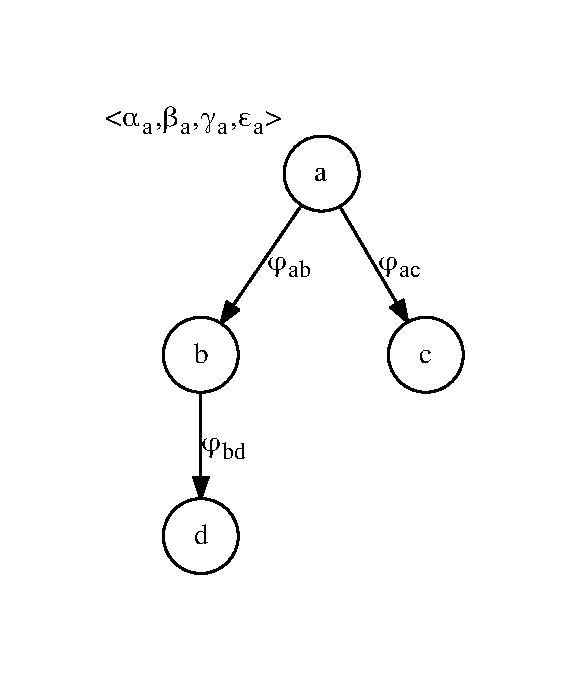
\includegraphics{fig/base-graph.eps}
\caption{The base item set graph, which includes item-specific paramters}
\end{figure}

\begin{figure}[!p]
\label{fig:student-graph}
  \centering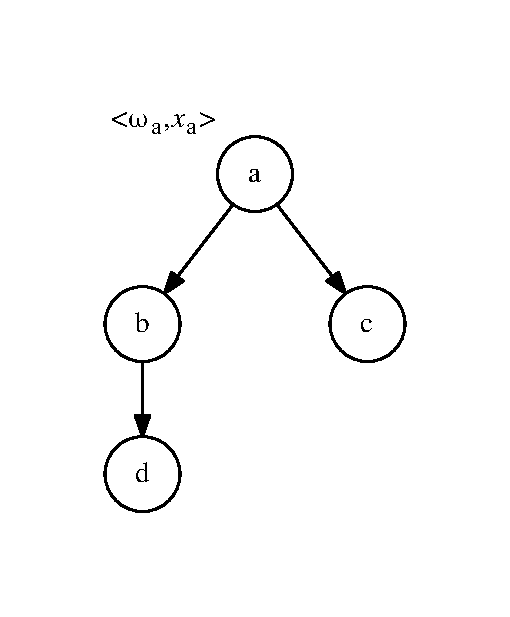
\includegraphics{fig/student-graph.eps}
\caption{The student-specific item set graph, which includes the list of
student responses and timestamps for each response}
\end{figure}

\subsection{Probability Estimates Using Dependees}

Logistic regression (pioneered by David Cox \cite{cox:1958}) is an ideal tool
for predicting success or failure given prior information about dependencies.
This is due to the fact that the dependent variable in question (the success of
answering a depender) is binary.  

One may wonder why any other form of regression technique is preferred over
linear regression.  Consider the linear equation in which a binary dependent
variable $Y$ depends on some response $X$:

\begin{equations}
         Y = a + bX + \epsilon
\end{equations}

where $a$ is some constant, $b$ is a coefficient, $\epsilon$ is the error, and
$Y$ assumes one of two possible values, 0 for failure or 1 for success.  Linear
regression has five assumptons, three of which are violated in this situation:

\begin{itemize}

  \item Linear relationship. Linear regressions require that linear
  relationships exist between the dependent variable and independent variables;
  however since the dependent variable assumes one of two possible values, the
  relationship is non-linear.

  \item Multivariate normality. This requirement holds that every linear
  combination of $k$ components has a univariate normal distribution.  This
  is not the case since each $k$ component assumes one of two possible values.

  \item Homoscedasticity. This requires that error terms along the regression
  are equal, but in the above situation, the variance of the error is dependent
  on the probability.   In particular $\mathrm{var}(\epsilon) = p(1-p)$.

\end{itemize} 

In addition, linear regressions require little to no multicollinearity; that
is, independent variables should be independent from one another; this may be
established by computing the correlation matrix for the independent variables.
Also, there should be no auto-correlation: $y_2$, the second observation,
should not depend on $y_1$.  This assumption is typically violated by time
series, but it is assumed to hold here because the dependent variables are
measured across students rather than time.  

Binary logistic regression assumes that:

\begin{itemize} 

 \item The dependent variable is binary,
 
 \item P(Y=1) is the probability that the event $Y$ occurs, 
 
 \item The model is fitted correctly, which means that there are no extraneous
 variables used in the regression, but that all variables are meaningful,

 \item That error terms should be independent; each observation should be
 independent, and little to no multicollinearity should exist.  

 \item Indepedent variables should be linearly related to the log odds of
 the event.

\end{itemize} 

It is important to note that the third assumption may or may not hold depending
on the correlations between the dependees.  The nature of the problem is such
that one expects dependee questions to be intercorrelated.  One possible remedy
is to group the questions to avoid intercorrelations.

Logistic regression is a regression of what are known as log odds. The odds
are defined as:

\begin{equations}
  \mathrm{odds} = \frac{p}{1-p}
\end{equations}

And the log odds, or logit, is defined as:

\begin{equations}
  \logit(y) = \ln(\mathrm{odds}) = \ln\Big(\frac{p}{1-p}\Big) = a + bX
\end{equations}

Correspondingly, odds may be defined as follows:

\begin{equations}
  \frac{p}{1-p} = e^{a + bx}
\end{equations}

Solving this equation for $p$ yields

\begin{equations}
  p = \frac{e^{a + bx}}{1 + e^{a + bx}}
\end{equations}

which can be reduced to 

\begin{equations}
  p = \frac{1}{1 + e^{-(a + bx)}}
\end{equations}

This is called the logistic curve, which is one in the family of sigmoid
curves.  It is identical to the type of curve used in Item Response Theory.
Compare the exponent in the Item Response Theory probability formula with 
the right-hand-side of the logit function:

\begin{equations}
  a + bx = \alpha(\beta - 1)\theta
\end{equations}

In the 2PL model, in which $\gamma_i$ is absent, the Item Response Theory
calculation of $\theta_s$ can be interpreted as a logistic regression in which
the unknown coefficient is $\theta_s$, the item-dependent inputs are given by
$\alpha(\beta-1)$, and the constant $a=0$.

Thus, a modified form of logistic regression may be sought.  It is desirable
to keep in account the item discrimination as well as the trait ability of
the student. 

\begin{equations}
  Y = b_1X_1 + b_2X_2 + \ldots + b_{n-1}X_{n-1} + b_n\alpha_i(\theta_s-\beta_i)
\end{equations}

In this expression, the term $\alpha_i(\theta_s-\beta_i)$ is retained, however
it is multiplied by a coefficient $b_n$ to determine its weight. Likewise
coefficients $b_1$, $b_2$, \ldots $b_{n-1}$ determine weights of the dependee
items.  This results in a probability function for answering the depender
question correctly given responses for the dependee questions:

\begin{equations}
  p = \frac{1}{1 + e^{b_1X_1 + b_2X_2 + \ldots + b_{n-1}X_{n-1} + b_n\alpha_i(\theta_s-\beta_i)}}
\end{equations}

To determine the individual contribution of each predictor (dependee), the
Wald statistic may be used.  It is defined as:

\begin{equations}
  W_i = \frac{b_i^2}{SE_{b_j}^2}
\end{equations}

If the statistic is sufficiently low, then the supposed dependee is likely not
a dependee at all, in which case the edge indicating the dependency
relationship may be pruned from the tree.  The logistic regression model will
naturally assign a low weight to such a dependee, and its use in the scheduling
algorithm will be limited by its relative weight.

\begin{figure}[!p]
\label{fig:neural}
  \centering\includegraphics[width=.6\textwidth]{fig/neural.eps}
\caption{A perceptron; a single-layer neural network, where the inputs a, b, and c
are multiplied by weights, summed, and applied to a sigmoid squash function}
\end{figure}

\begin{figure}[!p]
\label{fig:deps}
  \centering\includegraphics[width=.6\textwidth]{fig/deps.eps}
\caption{A view of the dependency graph and weights used in the logistic regression,
including the item parameters}
\end{figure}

The use of the logistic regression model in the intelligent tutoring system
suggests that the student would need to have answered all the dependencies
(that values of 0 or 1 are available).  In many instances where it is desirable
to use such a predictive model, this is not the case; instead what is available
is a probability that the student will be able to answer the question
correctly.  In such cases, the model is used with the probabilities calculated
using Item Response Theory.

The above probability estimates also assume an atemporal view of questions: if
the student has answered a question, the student remembers the answer to the
question permanently; however this is evidently not the case.  

What remains is a temporal account of questions, in particular the role of
memory and forgetting.



\pagebreak
\singlespacing
\chapter{Memory}
\doublespacing
\section{Models of Memory}

Ebbinghaus is credited with a theory of memory and forgetting which has
withstood empirical study for over a century \cite{ebbinghaus}. It is known as
the power law of forgetting.  According to the power law of forgetting, the
strength of a memory after a time $t$ falls off exponentially: 

\begin{equations}
\label{eq:ebbinghaus}
 S(t) = ae^{-bt}
\end{equations}

In this model, $a$ is the initial strength of the memory, and $b^{-1}$ is a
decay rate.  The curve drawn by this function is known as the curve of
forgetting, which is depicted in Figure~\ref{fig:forgetting}.  If $a=1$, the
function may be interpreted as a probability function:

\begin{equations}
\label{eq:ebbinghaus-p}
 p_{recall}(t) = e^{-bt}
\end{equations}

\begin{figure}[p!]
 \label{fig:forgetting}
 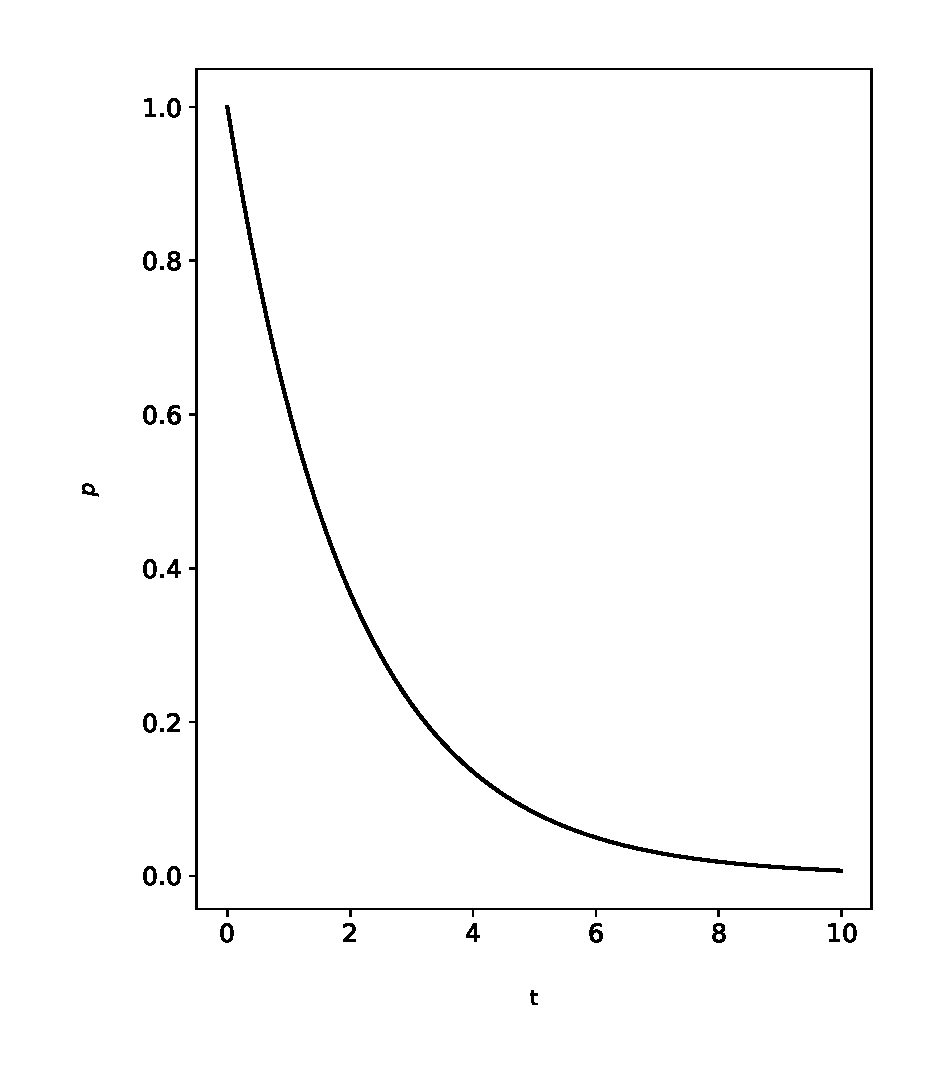
\includegraphics{fig/forgetting.eps} 
 \caption{The Ebbinghaus curve of forgetting, which features an exponential
 dropoff of memory strength over time}
\end{figure}

\begin{figure}[p!]
 \label{fig:modified}
 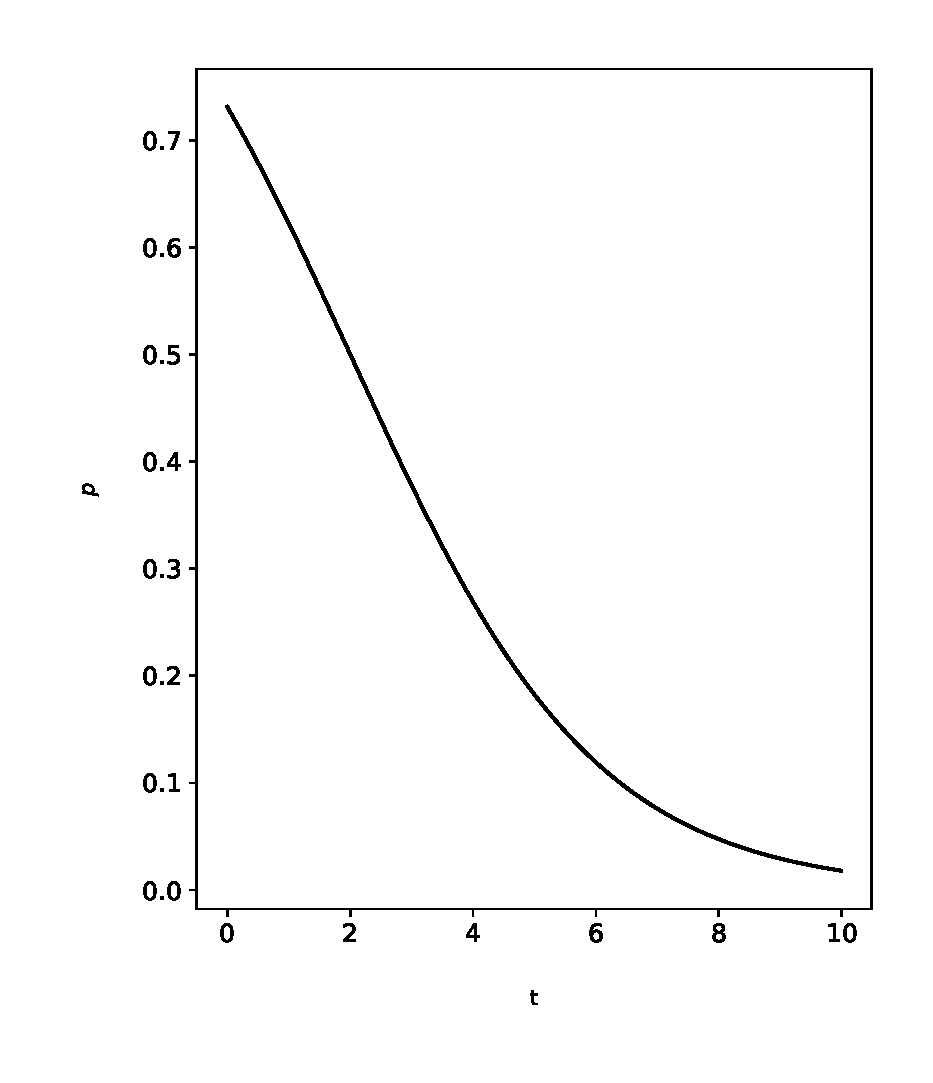
\includegraphics{fig/modified.eps} 
 \caption{The modified curve of forgetting, which resembles the reverse
 sigmoid function}
\end{figure}

According to the theory, if the memory strength falls below a certain
threshold, then in the absence of any intervening information (that is,
information which re-activates the memory via association), the individual will
be unable to spontaneously recall the information.  In a probabilistic model,
one may set the threshold at .5 probability---the probability below which the
individual has more than likely forgotten the information. 

\section{ACT-R}

As has been mentioned in Sec~\ref{sec:litreview}, John Anderson is credited
with having developed Adaptive Control of Thought-Rational (ACT-R), a
process-based model which simulates the solving of problems.  In ACT-R, there
are goals, akin to problem statements; and rules, or processes used to solve
problems; and finally facts, or knowledge utilized in the course of applying
rules. 

In addition to this, however, Anderson added models for memory and forgetting
to support realistic recall probabilities and latencies.  The memory component
is based on Ebbinghaus' model of memory retrieval.  Anderson added a component
to explain memory re-activation of a memory.  According to Anderson's model, a
chunk of memory $i$ is re-activated (or additionally activated) to the extent
that other chunks of information (related concepts, words, ideas, etc.) which
have some association to $i$ are attended to.  This notion is captured in the
following equation \cite{anderson2000implications}:

\begin{equations}
\label{eq:anderson-activation}
a_i = b_i + \displaystyle\sum_{i=j}^n w_j s_{ji}
\end{equations}

In this equation, known as the activation equation, the activation of a chunk
$i$ is equal to its base activation $b_i$, plus the products of the attentional
weights $w_j$ by the associative strength of $s_{ji}$ to other chunks.  This
provides an intuitive explanation for the manner in which recall of a target
chunk can be stimulated by dropping hints, using certain key words or phrases,
or mentioning related material. 

Practice has the effect of causing the base strength of the memory to increase,
and delays cause the strength of the memory to drop off
\cite{anderson2000implications}:  

\begin{equations}
\label{eq:anderson-spacing}
b_i = \mathrm{ln} \Bigg( \displaystyle\sum_{j=1}^n t_j^{-d} \Bigg)
\end{equations}

Here, $t_j$ is the time since the jth practice of an item, and $d$ is a decay
rate. \ldots

Some concepts, particularly the notion of re-activation of memories, have been
borrowed from ACT-R and modified to fit the more coarse-grained intelligent
tutoring system presented in this work.  In particular, total problems rather
than individial processes will have probabilities of recall associated with
them.  Also, associative strengths are established using a factor analysis.

\begin{figure}[p!]
 \label{fig:memory}
 %TODO: (SRB) the x-axis of this graph is messed up.
 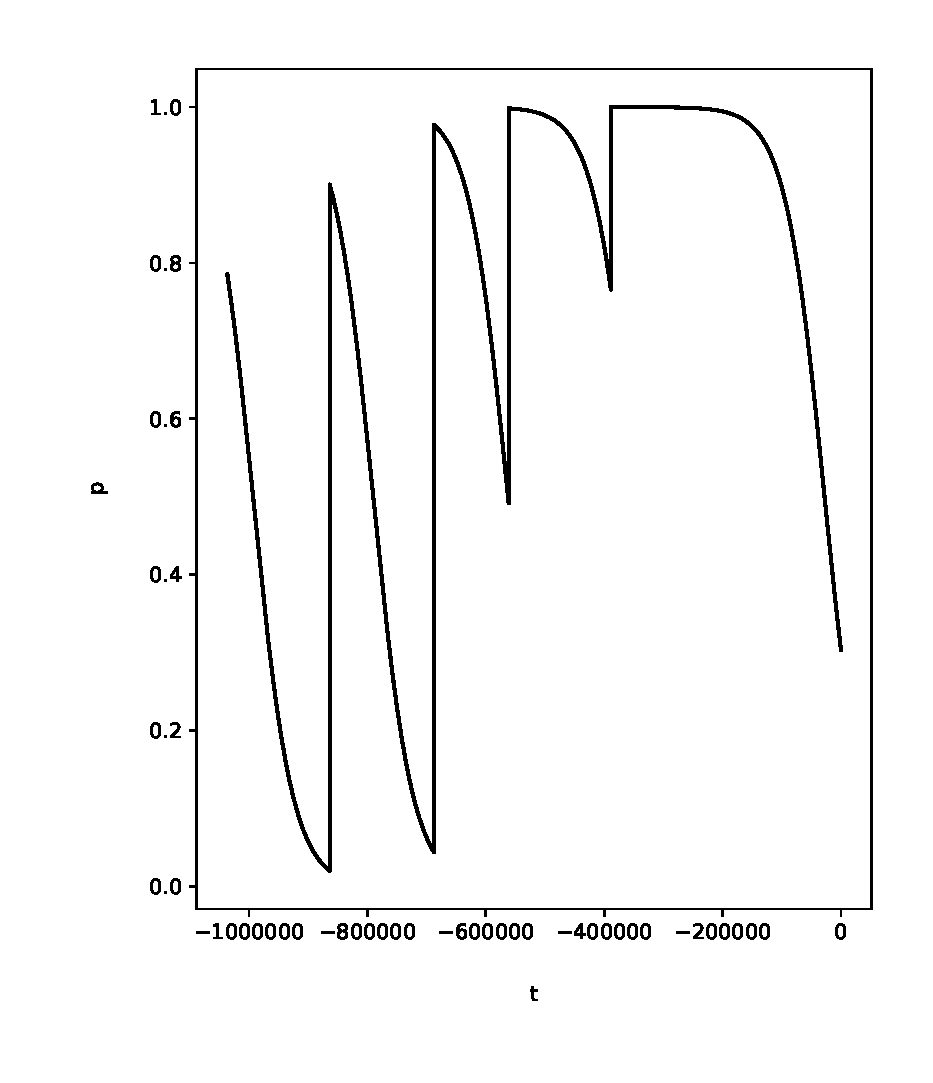
\includegraphics{fig/memory.eps} 
 \caption{Forgetting with re-activation; each spike in the graph is an
 additional trial where the student is exposed to the item again}
\end{figure}

\begin{figure}[p!]
 \label{fig:spacing}
 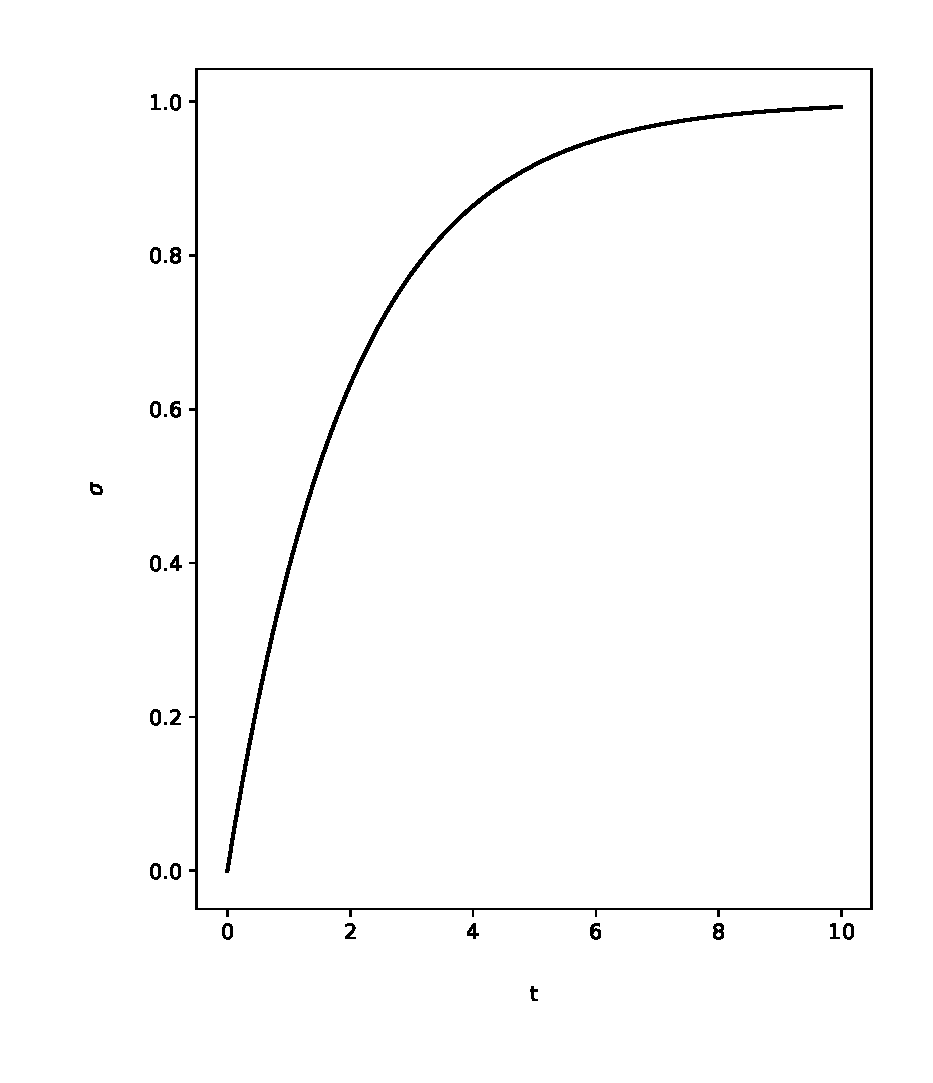
\includegraphics{fig/spacing.eps} 
 \caption{The learning curve, which indicates the extent of memory
 lifespan increase given a time between trials}
\end{figure}

\section{Alterations to Memory Model}

A slight modification to this theory accounts for short-term memory and
short-term memorization, which allows for a small time window for the student
to enjoy a high probability of recollection before dropping off sharply, as in
the original curve:

\begin{equations}
\label{eq:memory}
 p_{recall}(t) = \frac{1}{1 + e^{{m(t-\lambda)}}}
\end{equations}

In this equation, $\lambda$ is the lifespan of the memory; or, the amount of
time that passes until there remains only a .5 probability that the student
recalls the information.  The value $m$ is a parameter which controls the rate
of dropoff, much like the decay rate in Ebbinghaus' model.  An example curve
for this equation is given in Figure~\ref{fig:modified}.


\section{Re-Activation}
\label{sec:reactivation}

To account for re-activation, a simple model for the extension of half-life
may be used: 

\begin{equations}
\label{eq:lambda-rho}
 \lambda_n = \rho_s \lambda_{n-1}
\end{equations}

Here, $n$ refers to exposure or trial number $n$.  In the intelligent tutoring
system, this is the nth time that the student has seen the problem.
$\lambda_{n-1}$ is the former lifespan of the memory.  $\rho_s$ is a learning
rate, which is a parameter particular to the student; its domain is (1,
$\infty$].  The intuition captured by this formula is that with an increased
number of trials, the lifespan of the memory increases.

Apparently there is a difference in problems in the ease with which they are
learned.  An addendum to this can be used to account for individual differences
in problems: 

\begin{equations}
\label{eq:lambda-mu}
 \lambda_n = \mu_i \rho_s \lambda_{n-1}
\end{equations}

Here, $\mu_i$ represents the memorability of the problem, or the ease with
which the problem solution can be committed to memory. 

% TODO: relationship to power law of learning or learning curve.
% TODO: show relationship between Anderson and this?

\subsection{Spacing Effect}

The spacing effect is the effect that the amount of time in between trials has
on the memorization of a chunk of memory.  In the above model, memorization is
interpreted as an increase in the lifespan of a memory.  If only a short amount
of time passes between the last trial, the effect will not be as great as if a
longer time has passed.  One consequence of this is that, according to the
spacing effect hypothesis, cramming is ineffective (where cramming is namely
repeating trials in short bursts).

The spacing effect can be accommodated in the memory model used by the
intelligent tutoring system.  We define a function for the dropoff:

\begin{equations}
  \label{eq:spacing}
  \sigma_t = (1 - e^{-at})
\end{equations}

This indicates the extent to which the spacing from the time the item was last
seen influences the increase in the lifespan of the memory: 

\begin{equations}
\label{eq:lambda-final}
 \lambda_n = (1 + \sigma_t \mu_i \rho_s) \lambda_{n-1}
\end{equations}

The utility of this model is in assessing the probability with which a student
answers a question; not only based on trait ability and dependency
relationships, but also on the inherent tendency to forget information with the
passage of time.

It will be assumed that, if a student has been exposed to a item before, then
the probability of being able to answer the item correctly may assume one of
two values.  The first is based upon recollection; it is the probability of
recalling the facts, processes, and so forth required to produce the solution
for an item.  The second is based upon derivation of the solution from known
facts, processes, and so forth in the dependencies, as if the student were
answering the question for the first time.  That is, if a student does not
recall the process for solving a problem, the probability defaults to the
probability based upon item parameters, trait ability and dependency
relationships:

\begin{equations}
\label{eq:p-final}
p =\left\{
         \begin{array}{ll}
               p_{recall}(t) & \mathrm{if}\  p_{recall} > p({\theta_s, x_1, \ldots}) \\
               p({\theta_s, x_1, \ldots}) & \mathrm{otherwise}
         \end{array}
       \right.
\end{equations}

Now the intelligent tutoring system has models of dependency relationships
among questions and probability estimates for questions, and all other
mathematical equipment required to schedule problems. 




\pagebreak
\singlespacing
\chapter{Scheduling}
\doublespacing
\section{Item Scheduling}
\label{sec:scheduler}

The general procedure for scheduling content and assessments can be stated as
follows.  First, at the very beginning of the program, the trait ability matrix
for the student is initialized:

\begin{equations}
  \Theta \leftarrow -3
\end{equations}

That is, the algorithm initially proceeds on the assumption that it is unlikely
for any student to answer any question.  The initial estimate for the $\alpha$
values may be 1, such that the Item Response Theory 3PL model defaults to 2PL
in the absence of any data.  The initial difficulty estimates may be determined
by the instructor, or they may be initialized set to 0.  The $\mu$ values may
be initialized to 1.

The first iteration schedules a preliminary test consisting of a diagonal block
of the trait ability matrix, for example:

\begin{equations}
\Theta_s =\left[
         \begin{array}{llll}
              \y\theta_{s11} & \y\theta_{s21} & \y\theta_{s31} & \ldots \\
              \y\theta_{s12} & \y\theta_{s22} &                &        \\
              \y\theta_{s13} &                & \ddots          &        \\
              \vdots         &                &                 &        \\
         \end{array}
       \right]
\end{equations}

The test should be small enough to be feasible while having enough questions to
support an MLE.  At least two questions are needed per (Bloom $\times$ concept)
for an MLE.  Asking the questions from a single catetegory is sufficient to
jumpstart the process, but the larger the triangle, the richer the initial
information ($\alpha$, $\beta$ values).  Once the data is collected, it is then
possible to re-calculate $\alpha_i$ and $\beta_i$ for all items. 

With respect to $\alpha_i$, it is desirable to discard any question $i$ for
which $\alpha_i \leq 0$.  Recall that negative values of $\alpha$ indicate a
negative biserial correlation with the composite score, which means that the
question asked is an indicator of whether or not the student will perform
poorly on the overall measure.  

If $\alpha_i$ is close to -1, then the question may have predictive power, in
which case it should be analyzed for its properties.  It may be desirable to
retain such questions for the purpose of predicting success.  Regardless, if
$\alpha_i < 0$, then it along with its subtree should be severed from the
dependency graph.

With the response set, $\Theta_s$ can be constructed and the proximal zone of
development can be identified.

The roots of the assessment tree are traversed until either a question within
the neighborhood of the trait ability is found, or if no question is found, the
traversal ends and another random category is selected.

\subsection{Finding High-Impact Items}

Once a node on the tree is found, a check is performed to ensure the
dependencies have been asked.  If not, an in-order recursive descent is done on
each dependency, and this procedure is performed on the sub-dependencies.  If
all dependencies have been asked, the probability of the target question is
evaluated.  If the probability is .5, the question is asked. 

If the probability is less than .5, a confirmatory factor analysis is performed
on the dependencies of the node.  At any time, this factor analysis may reveal
a squared loading near zero, which indicates that the dependency relationship
indicated by the graph is not an actual dependency.  In that event, the link
between the target and the ``dependency`` is severed and a confirmatory factor
analysis is re-run on the remaining dependencies.

The most impactful dependency is sought.  This dependency item $i$ is selected
as follows: 

\begin{equations}
  \underset{i}{\mathrm{argmax}} \Bigg[ (1 - p_i) \lambda_i^2 \Bigg]
\end{equations}

The value $\lambda^2$ is the proportion of variance due to that dependency, so
it is preferred to start with higher proportions of variance.  Also $(1-p_i)$
is the room for improvement in the probability of the answering the dependency
correctly.  The intuition is that the more likely it is that the student is
able to answer the dependency correctly, the probability of answering the
target question rises---to the extent of the dependency relationship. 

\subsection{Finding the Next Item}

The maximal value for $(1 - p_i) \lambda_i^2$ may have $p_i < .5$, in which
case the above procedure is recursively applied to the dependencies with
$i$ as the target question.  

Eventually, the algorithm will converge on either a question for which $p_i >
.5$, or it will hit the leaves.  What this means is that there is no question
in the sub-tree for which $p_i$

\subsection{Finding the Whole Schedule}



\pagebreak
\singlespacing
\chapter{Experimental Results}
\doublespacing
\section{Experiments Supporting the Utility of the Taxonomy}

\textbf{Experiment 1}. Our first experiment tested to see if there is a
performance difference between computer-based assessment and paper-based
assessment when questions are ordered by Bloom level.  Our hypothesis was that
students taking the computer-based assessment would fare better than those
taking the paper-based assessment because of the immediate feedback offered by
the computer-based assessment.

We designed a test of 10 questions (2 concepts, each concept having questions
over 5 Bloom levels) to give to students\footnote{All questions may be viewed
at: https://steam.cct.lsu.edu/assessment/}. The questions were of
multiple-choice and short-answer format.  There were two knowledge,
comprehension, application, analysis, and evaluation questions.  No synthesis
questions were asked because of the constrained formats allowed by the
computer-based testing framework.  An interrater reliability of 90\% was
determined by two independent raters (the authors), both computer science
educators, who assessed the Bloom levels of the questions.  After a point of
disagreement about an evaluation-level problem, the test was adjusted to yield
an 100\% interrater reliability.

We designed a test of 10 questions (with 2 concepts, each concept having
questions over 5 Bloom levels) to give to students. The concepts tested were on
recursion and binary trees, and were written to be language-independent.  The
questions were of multiple-choice and short-answer format.  There were two
knowledge, comprehension, application, analysis, and evaluation questions.  No
synthesis questions were asked because of the constrained formats allowed by
the computer-based testing framework.  An interrater reliability of 90\% was
determined by two independent raters, both computer science educators, who
assessed the Bloom levels of the questions.  After a point of disagreement
about an evaluation-level problem, the test was adjusted to yield an 100\%
interrater reliability.

Evaluation-level problems are resistant to multiple-choice and short-answer
formats because of the nature of the category.  Our approach was to use
multiple-choice questions of the ``choose the best answer'' format, in which
there are many proposed uses of a concept or language construct, but one stands
out as the most sensible from the standpoint of experts. 

The test resembled a quiz that might be given in the normal course of teaching
the class. At the end of the quiz, the question ``how satisfied were you with
the (paper/computer)-based medium?'' was asked to gauge satisfaction
differences as well.

For this experiment, volunteers were recruited from a Java programming class
for introductory computer science students.  All students volunteered; candy
was offered as an incentive for all the experiments.  We split the classroom
into two groups, matched based on their current grade in the course.  We gave
the control group the paper quiz, and the experimental group the computer-based
quiz.

An answer was scored as totally correct if it coincided exactly with the
solution, and otherwise scored as incorrect. Correct answers were encoded with
1, incorrect with 0.  A composite score was derived by summing these scores
per-student.

\textbf{Experiment 2}.  The second experiment tested the effect of ordering the
questions by Bloom level.  For this experiment we designed another test of 10
questions (2 concepts, each concept having questions over 5 Bloom levels).
This test also covered recursion and binary trees. In the control condition,
questions were given in forward Bloom-level order.  In the experimental
condition, they were given in reverse order.

For both Experiments 2 and 3, participants were recruited in the same manner;
however for this experiment a C++ class which followed the same conceptual
track was also added to the pool. Matched-pairs were assigned to each group
bsaed on their current grade in each course.  The test was constructed and
interrater reliability gauged in the same manner, and the test was also scored
in the same manner.

\textbf{Experiment 3}. The third experiment tested the effect of intervening
questions on the performance of later questions in the assessment.  Our
hypothesis was that overall performance would be improved if incorrect answers
triggered the addition of new {\em intervention} questions from a lower Bloom
level.

Experiment 3 participants were recruited from a different class. The test was
this time language-dependent (MATLAB) and tested mastery of control structures,
in particular for-loops.  In the control condition, the control group was given
an assessment of 10 questions, with 2 questions per the first five Bloom
levels. The experimental group was given an adaptive measure.  If at any point
a student answered a question incorrectly, then a question at the next lowest
level was given.  This applied to all levels except knowledge.  So for example
if a student answered an application-level question incorrectly, a
comprehension-level question (related to the application-level question) was
scheduled before another application-level question of the same type.  The
experimental group thus had a a maximum of 4 additional questions asked for a
total possible 14-question test.

\section{Analysis and Results}

\textbf{Experiment 1}. The experimental condition ($N$=27 $M$=6.21) did in fact
show a higher mean score than the control condition ($N$=27 $M$=5.23) in
overall performance.  Statistical significance was tested with a one-tailed
two-sample matched-pairs Student's t-test on the composite score. The result
indicated a statistically significant difference ($t$=2.024, $p$=0.048).  The
experimental condition ($M$=4.93) showed a higher mean score than the control
condition ($M$=4.38) in satisfaction as well; a similar t-test was done and was
marginally statistically significant ($t$=1.7753, $p$=0.082).  


\textbf{Experiment 2}. The experimental condition ($N$=48, $M$=4.94) showed a
higher mean score than the control condition ($N$=48, $M$=4.31).  Statistical
significance was tested with a one-tailed parametric Student's t-test on the
composite score.  The result indicated a statistically significant difference
($t$=2.13, $p$=0.036).

\textbf{Experiment 3}. To tell the immediate effect of the intervention
questions, one-tailed parametric Student's t-test on the composite score of
questions starting after the first intervention question was done. It was
hypothesized that the experimental condition would perform better on the
remainder of the test. The experimental group ($N$=45, $M$=6.98) outperformed
the control group ($N$=45, $M$=6.23).  The result indicated a marginally
statistically significant difference ($t$=1.7082, $p$=0.092).

\subsection{Limitations}

A few validity concerns are to be pointed out. No random order was given in
Experiment 2 because of a lack of available subjects; hence it cannot be
inferred that forward order is no different from random order. The
experimenters (paper authors) designed the tests. The number of items per test
was small to allow for a conservative testing time.  For Experiment 1,
confounding variables (those other than immediate feedback) may have played a
role in test-taking because the test-taking media were different.


\section{Experiments Supporting the Reconciliation of the Taxonomy with IRT}

\subsection{Experiment 1}

\textbf{Experiment 1 Design}. In the first experiment, a selection of 16
multiple-choice questions on topics in operating systems concepts were asked to
a sample group of students (N=54) in an undergraduate-level operating systems
class.  Each question had 5 choices ($\gamma$=.2). These questions were tagged
with Bloom levels, and interrater reliability was calculated between two
independent raters with experience in curricular and course design.  Questions
were tagged with hypothesized difficulty levels, which were targeted to be
inversely proportional to the Bloom levels.  Hence the question author intended
for the knowledge questions to be difficult relative to analysis questions,
while still maintaining the appropriate Bloom category.


\textbf{Analysis of Experiment 1 Data}.  Interrater reliability on Bloom levels
was calculated to be 93\%.  Means for each Bloom level are reported below.
Clearly

\begin{center}
\begin{tabular}{|l|l|l|l|l|}
                                                                 \hline
      &   Knowledge & Comprehension & Appplication & Analysis \\ \hline
 $M$  &  .42 & .53 & .67 & .82  \\ \hline
\end{tabular}
\end{center}

One-tailed Student t-tests were performed on the three consecutive pairs of
means.  The mean for comprehension was statistically significantly greater than
the mean for knowledge ($t=2.00$), the same held true for application and
comprehension ($t=2.33$), and analysis and application ($t=2.64$).  These
statistics, in conjunction with the interrater reliability for the assignment
of Bloom levels, support the view that Bloom level and difficulty are
distinguishable.

In light of this data, a modification of IRT was sought in order to account for
the dependency relationships that existed among the questions.  Intuitively,
this modification of $p_i$ should possess the properties that: (a) if a
question $x_j$ is unrelated, $p_i$ should be unaffected; and (b) if $x_j$ is
fully related, $p_i$ should be equal to the response value for $x_j$. 

The degree of relationship may be expressed with Pearson's $r$, where
$r_{ij}=0$ indicates no relationship between $x_i$ and $x_j$ and $r=1$
indicates a full positive correlation.  An even more viable metric is the
coefficient of determination $r^2$, which indicates the proportion of variance
in the depender which is attributable to the dependee.  Intuitively, it is this
proportion of the probability which should be associated with the correctness
of $j$.  The remainder may be left to item response theory.  In the event of a
negative correlation, the response should be opposite.


\begin{align*}
  p_i(\theta) &=& (1-r^2) & \Big(\gamma_i + \frac{1-\gamma_i}{1+e^{\alpha_i(\theta-\beta_i)}}\Big) \\
              &+& (r^2)   & \Big(\mathbf{sgn}(r)x_{sj}+\frac{1-\mathbf{sgn}(r)}{2}\Big)
\end{align*}

The above formula satisfies our needs.  The \textbf{sgn} function gives the
sign of $r$.  For $r=1$, $p_i$ defaults to the correctness of the dependee's
answer (0 or 1, depending on whether or not the dependee was answered
correctly);  and for $r=-1$, $p_i$ assumes the flip of the dependee's answer.
For $r=0$, $p_i$ assumes the form of original IRT.  

In the MLE estimation of $\theta$, we would omit question $j$, since it is
included already in the above formula.

\subsection{Experiment 2}

\textbf{Experiment 2 Design}.  To test this modified theory, another experiment
was conducted.  The purpose of this experiment was to explore the relationship
among the probability predicted by unmodified IRT, the probability predicted by
modified IRT, and the correctness of the actual response.  It was hypothesized
that modified IRT should produce a more accurate output than unmodified due to
its account of dependency relationships.

As in the first experiment, a selection of 16 multiple-choice questions on
topics in operating systems concepts were asked to the same sample group of
students (N=54) in the same manner ($\gamma$=.2).  The questions covered 4
concepts, and each concept had 4 questions, each of different Bloom levels
(Knowledge, Comprehension, Application, Analysis), where each question of a
Bloom level higher than Knowledge was dependent on a question of an
immediately-lower Bloom level (e.g. the Application question was dependent on
the Comprehension question of the same concept).  These questions were asked in
forward Bloom order.  The hypothesized difficulties were held equal across
Bloom levels.


\textbf{Analysis of Experiment 2 Data}. \ldots Interrater reliability on Bloom
levels was once again calculated to be 93\%. 

\begin{center}
\begin{tabular}{|l|l|l|l|l|}
                                                                 \hline
      &   Knowledge & Comprehension & Appplication & Analysis \\ \hline
 $M$  &  .78 & .62 & .48 & .41  \\ \hline
\end{tabular}
\end{center}


To test the hypothesis that modified IRT leads to an increase in accuracy,
a t-test on the increase in accuracy of probability was conducted at the
.05 significance level.

First the probabilities $p_i^{irt}(\theta)$ (for original IRT) and
$p_i^{mod}(\theta)$ (for modified IRT) were calculated.  Note that each of
these formulas require $\theta$. The value for $\theta$ was calculated
per-student using the MLE method on the first data set.  To determine whether
or not $p_i^{mod}(\theta)$ was on the whole more accurate than $p_i^{irt}$, the
result

\[
  \Delta p_{si} = (2x_{si}-1) (p_i^{mod} - p_i^{irt})
\]

was calculated. Here $p_{si}$ represents the probability that student $s$ will
answer item $i$ correctly.  Then $\Delta p_{si}$ represents the increase in
accuracy of the probability; for example, it is positive if $p_i^{mod} >
p_i^{irt}$ and $x_{si} = 1$.

Finally, to test the effectiveness of $p_i^{mod}$, a one-tailed Student's
t-test was calculated on $\Delta p_{si}$ for the dependee questions (N=648).
The test revealed that $\Delta p_{si}$ is statistically significantly greater
than zero ($t=2.05$), implying that $p_i^{mod}$ indeed produces a more accurate
estimate than IRT alone. 

As the data reveals, the proportion of students who passed a question did not
agree with the hypothesized difficulties.  It was suspected that this may be
due to the effect of item dependencies, which the next experiment investigates
in further detail.

\subsection{Experiment 3}

\textbf{Experiment 3 Design}.  One question remains: can $p_i^{mod}$ be used in
some meaningful way?  Suppose we wish to maximize the probability that a
student answers an Analysis question correctly, and that this Analysis question
depends on an Application question.  For that matter, it may depend on more
questions, each of which having its own degree of relatedness to the depender.

We thus posit a more general form of modified IRT which takes into account
multiple dependencies using factor analysis \cite{kim1978}.  From a factor
analysis, it is possible to obtain the proportion of variance explained by each
dependency by squaring the factor loading.  A factor analysis was performed on
the dependent question using dependees as factors to obtain these proportions
of variance explained.

Those proportions of variance could then be used as part of a more generalized
modification to IRT:

\begin{align*}
  p_i(\theta) &=& (1- (\displaystyle\sum_j v_j)) & \Big(\gamma_i + \frac{1-\gamma_i}{1+e^{\alpha_i(\theta-\beta_i)}}\Big) \\
              &+& \displaystyle\sum_j (v_j)   & \Big(\mathbf{sgn}(r)x_{sj}+\frac{1-\mathbf{sgn}(r)}{2}\Big)
\end{align*}

In this generalized formula, $v_j$ refers to the proportion of variance
explained by the dependee $j$ (the squared factor loading for $j$).  Therefore
the sum of these is the total explained variance; one minus the sum is the
total unexplained variance.  Intuitively the probability is proportional to the
amount of variance explained by a dependee.  On the one hand, if one dependee
explains 90\% of the total variance, and the student answers this dependee
correctly, the probability should depend heavily on whether or not the dependee
was correct.  On the other hand, if the total unexplained variance is 1, this
would imply the dependees are not dependees at all.  In this case, the
probability defaults to the item response theory calculation, which uses the
best available information (trait ability and question parameters).

In our experiment to test the utility of this formula, we first required a
small problem set with one depender and multiple dependees.  The experiment
was intended to test whether or not the asking of highly-dependent questions
increased mean scores.

For this we first required proportions of variance between depender and
dependees.  We created 4 questions, where the 4th question had three dependees.
We then asked some of our students (N=22) to answer all of these questions to
obtain proportions of variance, which are listed below.  

\begin{center}
\begin{tabular}{|l|l|l|l|l|}
                                  \hline
      &   q1 &  q2  & q3 & q4  \\ \hline
$v_j$ &  .02 & .23 & .30 &     \\ \hline
 M    &  .67 & .66 & .43 & .34 \\ \hline
\end{tabular}
\end{center}

The others would receive a combination of questions.  Each student was randomly
assigned to one of eight groups.  Four students received each combination of
three questions, such that 4 received the depender outright, 12 received one of
the three dependees (4 each) before the depender, 12 received two of the three
dependees (6 each) prior, and 4 received all three dependees.  The purpose of
this was to test the effect of exposure of each dependee.  Thus each dependee
question appeared in half of the students' assessments.  The total number of
respondents for the depender was 32, and the total number of respondents for
each dependee was 16.  

\textbf{Analysis of Experiemnt 3 Data}.  The analysis of this data required
examining the relationship between dependent response and dependee exposure.

Let $E_{sj}$ be 1 if student $s$ was exposed to $j$, 0 otherwise.  Then, our
hypothesis was that exposure of dependee questions should result in an increase
in the probability that the student answers the depender correctly, in
proportion to the amount of variance explained by the dependee.  Below in the
table is the number of times the depender was answered correctly given
exposure to a set of dependees.  Though the data set is small, there does
appear to be a trend in the data.  A clearer trend can be observed by summing
the number of correct responses per exposure to a given question.

\begin{center}
\begin{tabular}{|l|l|l|l|l|}
\hline
dependees    & \#correct &  percent & \#correct & percent \\ \hline
none         &  1  & .25  &1&  .06 \\ \hline
q1           &  1  & .25  &8&  .50 \\ \hline
q2           &  2  & .50  &10& .62 \\ \hline
q3           &  3  & .75  &11& .69 \\ \hline
q1, q2       &  2  & .50  && \\ \hline
q1, q3       &  2  & .50  && \\ \hline
q2, q3       &  3  & .75  && \\ \hline
q1, q2, q3   &  3  & .75  && \\ \hline
\end{tabular}
\end{center}

The table shows the percent of students who answered the depender correctly
given a particular set of questions (left), as well as the percent of students
who answered the depender correctly given exposure to a given question (right). 
It is interesting to note that to an extent, the proportions of variance
explained by a given question appear to be co-related to the percentage of
students who answered the depender correctly.  However, the numbers are too
small to draw a definitively conclusion.

Due to the low $N$ in Experiment 3, the results do not present
\emph{conclusive} evidence that the intervention of the dependee questions was
responsible.  However, there is enough preliminary evidence to warrant further
investigation.  If there is an effect, it is suspected that exposure to the
dependee problem solution by the ITS plays a larger role than simply the
question itself.


\section{Experiment Supportng the Utility of the Scheduler}

\pagebreak
\singlespacing
\chapter{Executability and Reporting}
\doublespacing
\section{Executability Component}


\pagebreak
\singlespacing

%To insert additional chapters, copy the previous five lines, using chapterX as the argument of the 
%\input command for Chapter X, where X=6,7,8,...
\addtocontents{toc}{\vspace{12pt}}
\addcontentsline{toc}{chapter}{\hspace{-1.6em} REFERENCES}
%\begin{thebibliography}{999}
%\vspace{0.9em}
%% Duplicate of my research, more importantly suggests outright that Bloom=difficulty
@article{newman1988effect,
  title={Effect of varying item order on multiple-choice test scores: Importance of statistical and cognitive difficulty},
  author={Newman, Dianna L and Kundert, Deborah K and Lane Jr, David S and Bull, Kay Sather},
  journal={Applied Measurement in education},
  volume={1},
  number={1},
  pages={89--97},
  year={1988},
  publisher={Taylor \& Francis}
}


% Very clear support for the thought that Bloom=difficulty, even used for course difficulty rating
@inproceedings{oliver2004course,
  title={This course has a Bloom Rating of 3.9},
  author={Oliver, Dave and Dobele, Tony and Greber, Myles and Roberts, Tim},
  booktitle={Proceedings of the Sixth Australasian Conference on Computing Education-Volume 30},
  pages={227--231},
  year={2004},
  organization={Australian Computer Society, Inc.}
}


% Very clear support for the thought that Bloom=difficulty
@article{lord2007moving,
  title={Moving students from information recitation to information understanding: exploiting Bloom's taxonomy in creating science questions},
  author={Lord, Thomas and Baviskar, Sandhya},
  journal={Journal of College Science Teaching},
  volume={36},
  number={5},
  pages={40},
  year={2007},
  publisher={National Science Teachers Association}
}


% Support for people thinking that Bloom=difficulty
@inproceedings{johnson2006bloom,
  title={Is Bloom's taxonomy appropriate for computer science?},
  author={Johnson, Colin G and Fuller, Ursula},
  booktitle={Proceedings of the 6th Baltic Sea conference on Computing education research: Koli Calling 2006},
  pages={120--123},
  year={2006},
  organization={ACM}
}


% Support for people thinking that Bloom=difficulty
@inproceedings{fuller2007developing,
  title={Developing a computer science-specific learning taxonomy},
  author={Fuller, Ursula and Johnson, Colin G and Ahoniemi, Tuukka and Cukierman, Diana and Hern{\'a}n-Losada, Isidoro and Jackova, Jana and Lahtinen, Essi and Lewis, Tracy L and Thompson, Donna McGee and Riedesel, Charles et al.},
  booktitle={ACM SIGCSE Bulletin},
  volume={39:4},
  pages={152--170},
  year={2007},
  organization={ACM}
}



% Support for Bloom!=difficulty: facility versus complexity
@article{hill1981testing,
  title={Testing the simplex assumption underlying Bloom's Taxonomy},
  author={Hill, PW and McGaw, B},
  journal={American Educational Research Journal},
  volume={18},
  number={1},
  pages={93--101},
  year={1981},
  publisher={Sage Publications}
}


% Support for Bloom!=difficulty
@inproceedings{thompson2008bloom,
  title={Bloom's taxonomy for CS assessment},
  author={Thompson, Errol and Luxton-Reilly, Andrew and Whalley, Jacqueline L and Hu, Minjie and Robbins, Phil},
  booktitle={Proceedings of the tenth conference on Australasian computing education-Volume 78},
  pages={155--161},
  year={2008},
  organization={Australian Computer Society, Inc.}
}



% Cursory
@article{sitthisak,
  title={Cognitive Assessment Applying with Item Response Theory},
  author={Sitthisak, Onjira and Soonklang, Tasanawan and Gilbert, Lester},
  journal={19th Annual International Conference on Computers in Education},
  year={2011}
}


% Bloom original
@book{bloom1956,
  title={Taxonomy of educational objectives},
  author={Bloom, Benjamin Samuel et al.},
  year={1956},
  publisher={David McKay}
}


% Factor analysis
@book{kim1978,
  title={Factor analysis: Statistical methods and practical issues},
  author={Kim, Jae-On and Mueller, Charles W},
  volume={14},
  year={1978},
  publisher={Sage}
}


% Newton Raphson
@book{baker2004,
  title={Item response theory: Parameter estimation techniques},
  author={Baker, Frank B and Kim, Seock-Ho},
  year={2004},
  publisher={CRC Press}
}


% R can be hooked to paper manuscripts to re-generate scientific findings.
@article{ castleberry2011,
          author    = {Dennis Castleberry}
         ,title     = {The Prickly Pear Archive}
         ,journal   = {ICCS}
         ,address   = {Singapore}
         ,publisher = {Elsevier}
         ,year      = {2011}
}


% ...26 studies were deemed as relevant. The main findings from these studies
% are: i) Bloom’s taxonomy has mostly been applied at undergraduate level for
% both design and assessment of software engineering courses; ii) software
% construction is the leading SE subarea in which Bloom’s taxonomy has been
% applied. The results clearly point out the usefulness of Bloom’s taxonomy in
% the SE education context.
@article{ britto2015,
   author = {Ricardo Britto and Muhammad Usman}
  ,title  = {Bloom’s Taxonomy in Software Engineering Education: A Systematic Mapping Study}
  ,journal= {Frontiers in Education Conference}
  ,address= {El Paso, TX}
  ,publisher= {IEEE}
  ,year   = {2015}
}


% Feedback from the students from both first year and second year reflected a
% positive response concerning their perception of the level on which the
% questions were asked. Regarding the first question, 381 students felt that by
% asking questions on higher levels of Bloom’s taxonomy it enriched their
% learning
@article{ bruyn2011
  ,author = {E de Bruyn and E Mostert and A van Schoor}
  ,title  = {Computer-based testing--the ideal tool to assess on the different levels of Bloom’s taxonomy}
  ,journal= {Interactive Collaborative Learning}
  ,address= {Piesany, Slovakia}
  ,publisher= {IEEE}
  ,year   = {2011}
}

% Bloom's taxonomy as applied to program comprehension was successful
@article{ buckley2003
  ,author = {Jim Buckley and Chris Exton}
  ,title  = {Blooms’ Taxonomy: A Framework for Assessing Programmers’ Knowledge of Software Systems}
  ,journal= {International Workshop on Program Comprehension}
  ,address= {}
  ,publisher= {IEEE}
  ,year   = {2003}
}

% Clustering of tasks using EEG is possible
@article{ chatterjee2015,
   author = {Debatri Chatterjee and rajat Das and Anirhudda Sinha and Shreyasi Datta}
  ,title  = {Analyzing Elementary Cognitive Tasks with Bloom's Taxonomy using Low Cost Commercial EEG device} 
  ,journal= {International Conference on Intelligent Sensors, Sensor Networks and Information Processing (ISSNIP)}
  ,address= {}
  ,publisher= {IEEE}
  ,year   = {2015}
}

% Preference for higher-order cognitive activities
@article{ goel2004,
   author = {Sanjay Goel and Nalin Sharda}
  ,title  = {What do engineers want? Examining engineering education through Bloom's taxonomy}
  ,journal= {Australasian Association for Engineering Education}
  ,address= {}
  ,publisher= {}
  ,year   = {2004}
}


% Context-aware vs. lexical schema
% Successful application to system
@article{ kelly2006,
   author = {Tara Kelly and Jim Buckley}
  ,title  = {A Context-Aware Analysis Scheme for Bloom's Taxonomy}
  ,journal= {International Conference on Program Comprehension}
  ,address= {}
  ,publisher= {IEEE}
  ,year   = {2006}
}

% several points aobut requirements
%  formal language
%  typing system
%  Bloom's semantics
@article{ loria-saenz2008,
   author = {Carlos Loria-Saenz}
  ,title  = {On Requirements for Programming Exercises from an e-Learning Perspective}
  ,journal= {}
  ,address= {}
  ,publisher= {}
  ,year   = {2008}
}

% increase in motivation
% comprehension testing fosters code reading
@article{ losada2008
  ,author = {Isidoro Hern\'{a}n-Losada}
  ,title  = {Testing-Based Automatic Grading: A Proposal from Bloom’s Taxonomy}
  ,journal= {International Conference on Advanced Learning Technologies}
  ,address= {}
  ,publisher= {IEEE}
  ,year   = {2008}
}

% speaks well for bloom's taxonomy when manually implemented
@article{ mahmood2014
  ,author = {Mahmood Niazi}
  ,title  = {Teaching global software engineering: experiences and lessons learned}
  ,journal= {IET Software}
  ,address= {}
  ,publisher= {}
  ,year   = {2014}
}

% speaks well for use of Bloom's taxonomy in software inspection
@article{ mcmeekin2009
  ,author = {David McMeekin and Brian von Konsky and Elizabeth Chang and David Cooper}
  ,title  = { }
  ,journal= { Conference on Software Engineering Education and Training }
  ,address= {}
  ,publisher= {IEEE}
  ,year   = {2009}
}

% good for novice programmers to dial it down
@article{ shuhidan2011
  ,author = {Shuhaida Shuhidan and Margaret Hamilton and Daryl D'Souza }
  ,title  = { Understanding Novice Programmer Difficulties via Guided Learning }
  ,journal= {ITiCSE}
  ,address= {Darmstadt, Germany}
  ,publisher= {ACM}
  ,year   = {2011}
}


% My last paper
@inproceedings{castleberry2016effect,
  title={The Effect of Question Ordering Using Bloom's Taxonomy in an e-Learning Environment},
  author={Castleberry, Dennis and Brandt, Steven R},
  booktitle={International Conference on Computer Science Education Innovation \& Technology (CSEIT). Proceedings},
  pages={22},
  year={2016},
  organization={Global Science and Technology Forum}
}


%\end{thebibliography}
\doublespacing
\bibliographystyle{plain}
\bibliography{mainfile}

\pagebreak
\singlespacing
\addtocontents{toc}{\vspace{12pt} \hspace{-1.8em} APPENDIX \vspace{-1em}}
\appendix
\chapter{Appendix A: Algorithms}
\vspace{0.5em}
\input{appendixA}
\pagebreak
\chapter{Appendix B: Mathematics}
\vspace{0.5em}
\input{appendixB}
\pagebreak
%If you need to insert additional appendices, copy the previous four lines, using appendixY as the
%argument of the \input commnd for Appendix Y, for Y=C,D,E,...

%Finally, the vita section is created and included in the Table of Contents.
\chapter*{Vita}
\doublespacing
\setlength{\parindent}{1.75em}
\vspace{0.2em}
\addtocontents{toc}{\vspace{12pt}}
\addcontentsline{toc}{chapter}{\hspace{-1.5em} VITA}
Insert the text of your vita, which is basically a description of yourself and your academic career.


\end{document}





